\section {Implementacja sprzętowa}
\subsection {Wykaz urządzeń}

W implementacji wykorzystane zostały następujące urządzenia:

\begin{enumerate}
\item Dalmierz Laserowy TFMini Plus UART/I2C
\item Silnik Krokowy 42HM48-1206 400 kroków
\item Arduino Uno
\item Sterownik A4988 model: STSPIN220
\item Zasilacz Laboratoryjny Zhaoxin RXN-305D
\item Zestaw przewodów
\item Płytka stykowa
\item Metalowe uchwyty dalmierza
\item Libela poziomicy
\end{enumerate}

\subsection {Specyfikacje urządzeń}
Implementacja wymagała zakupu i podłączenia ze sobą kilku urządzeń. Niektóre z nich zostały dobrane pod kątem wyjątkowych parametrów, inne były jedynymi z wielu spełniających wymagania projektowe. Poniżej zebrałem najistotniejsze argumenty za wyborem tych właśnie urządzeń.\\

\textbf{Dalmierz Laserowy TFMini Plus UART/I2C}\\
Dalmierz laserowy działający dla odległości od 0.1 do 12 metrów. Dokładność wynosi 5 cm (więcej w rozdziale o nepewnościach pomiarowych). Zasilany napięciem 5V. Komunikacja możliwa prze UART oraz I2C. Długość fali 850 nm. Częstotliwość pracy: od 1 Hz do 1000 Hz. Wymiary: 35 x 21 x 18,5 mm. Masa: 11 g.\\

\textbf{Silnik Krokowy 42HM48-1206}\\
Silnik wybrany ze względy na wysoką rozdzielczość - 400 kroków przy pełnym obrocie. Wadą był niski prąd zasilania (4.0V) co zawęziło wybór modelu sterownika. Unipolarny, sześcio przewodowy. Pobiera prąd 1200 mA na cewkę. Moment wynosi 3,17 kg*cm (0,31 Nm). Wymiary to 42 x 42 x 48 mm (NEMA 17).\\

\textbf{Arduino Uno}\\
Arduino Uno Rev3 - Uniwersalny moduł od Arduino Uno z mikrokontrolerem AVR ATmega328. Posiada 32 kB pamięci Flash, 2 kB RAM, 14 cyfrowych wejść/wyjść, 6 wejść analogowych oraz popularne interfejsy komunikacyjne. Wykorzystałem w projekcie ze względu na prostą obsługę, wysoką dostępność bibliotek oraz doświadczenia zdobyte podczas studiów.\\

\textbf{Sterownik A4988 model: STSPIN220}\\
Strerownik na bazie popularnego chipsetu A4988. Model wybrany ze względu na współpracę w silnikami niskoprądowymi (4.0 V).\\

Schemat:\\
\begin{figure}[h]
    \centering
    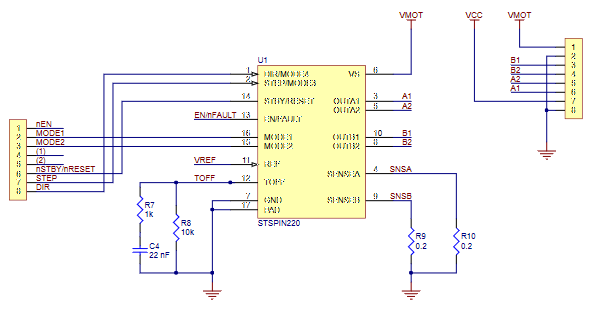
\includegraphics[scale=0.6]{a4988_scheme}
    \caption{Schemat modelu STSPIN220}
    \label{fig:a4988_scheme}
\end{figure}

\textbf{Zasilacz Laboratoryjny Zhaoxin RXN-305D 30V 5A}\\
Stabilizowany zasilacz laboratoryjny z płynną regulacją napięcia w zakresie od 0 do 30 V oraz prądu w zakresie od 0 do 5 A. Zasilacz jest chłodzony wentylatorem, co umożliwia jego prace w trybie ciągłym.
\begin{figure}[h]
    \centering
    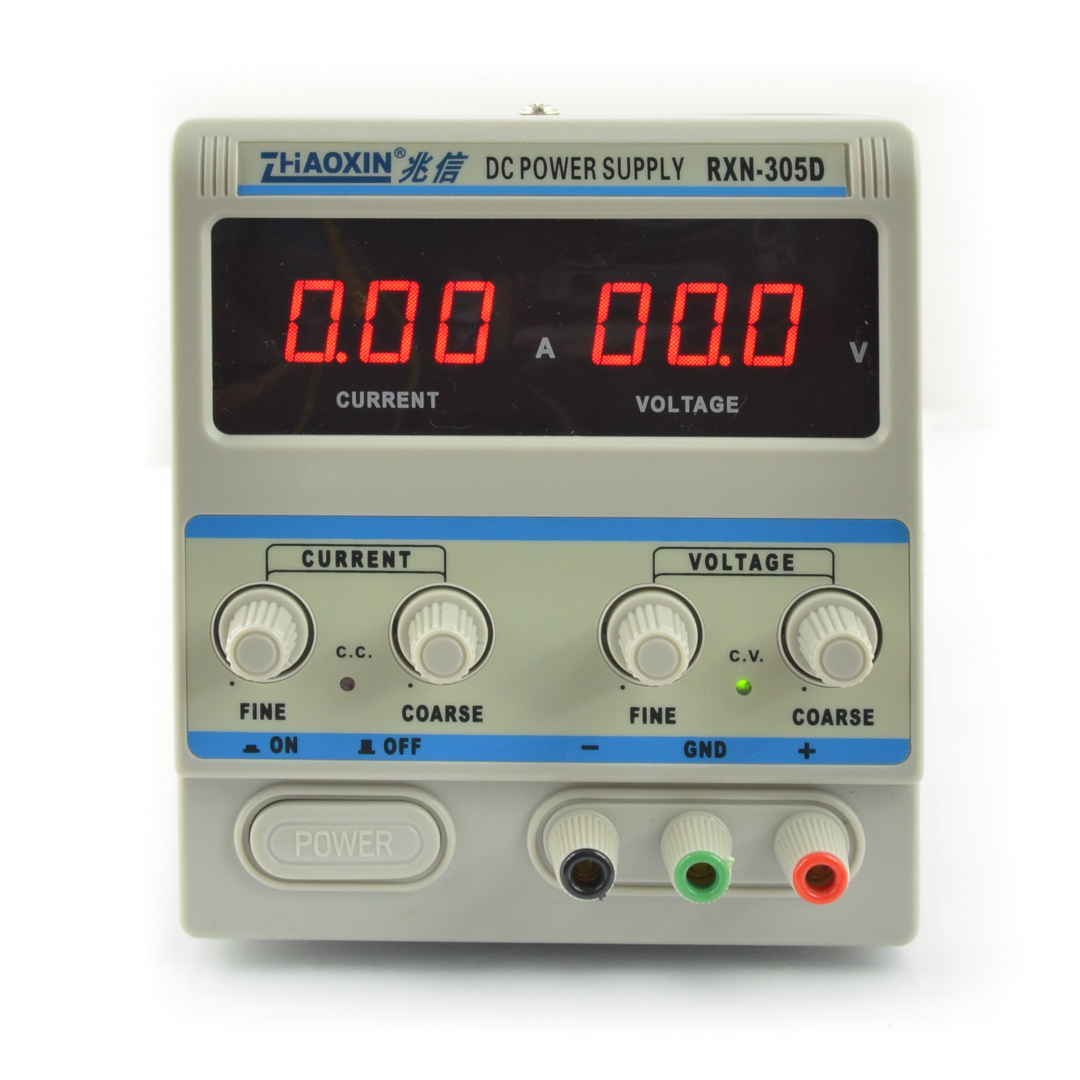
\includegraphics[scale=1.0]{zhaoxin_front_panel}
    \caption{Panel frontowy zasilacza Zhaoxin RXN-305D}
    \label{fig:zhaoxin_front_panel}
\end{figure}


\textbf{Zestaw przewodów}\\
Wielokolorowe przewody o długości 20 cm zakończone złączami męskimi.\\

\textbf{Metalowe uchwyty dalmierza}\\
Wykonane przeze mnie uchwyty z metalowych elementów starych mebli. Uchwyt służył stabilnemu umiejscowieniu dalmierza na obrotowej części silnika krokowego. Po wykonaniu uchwytu jego wymiary, katy i precyzja wykonania sprawdzone zostały suwniarką. Uchwyt ma również możliwość umieszczenia libel poziomicy.
\begin{figure}[h]
    \centering
    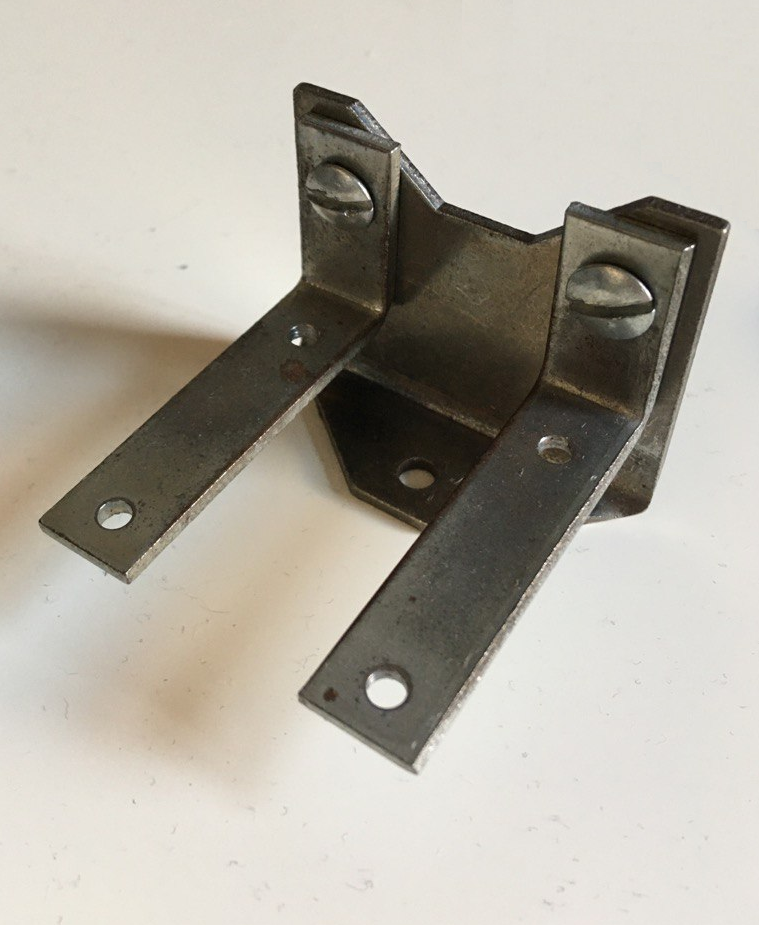
\includegraphics[scale=0.25]{uchwyt}
    \caption{Metalowy uchwyt dalmierza}
    \label{fig:uchwyt}
\end{figure}

\textbf{Libele poziomicy}\\
Tanie libele poziomicy od średnicy 15 mm i wysokości 7 mm. Zakupione w serwisie Allegro, ich dokładność jest mocno dyskusyjna ale pozwalały one w przybliżonym stopniu ocenić poziom zarówno podłoża jak i dalmierza umiejscowionego na uchwycie.

\begin{figure}[h]
    \centering
    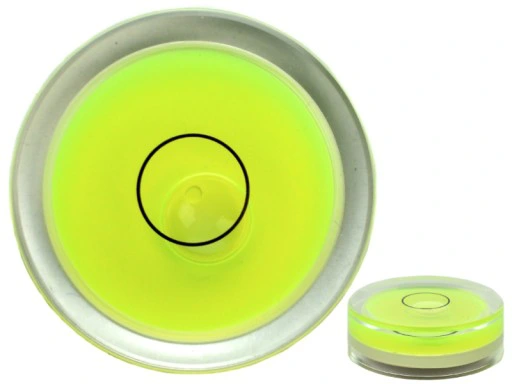
\includegraphics[scale=0.25]{libela}
    \caption{Libela poziomicy 15mm}
    \label{fig:libela}
\end{figure}

\begin{figure}[h]
    \centering
    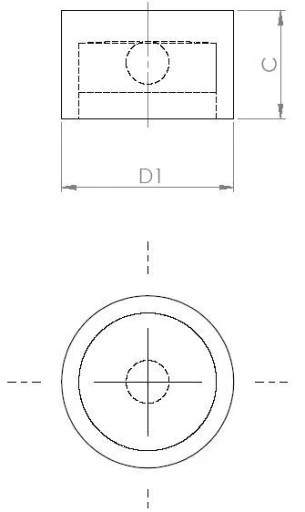
\includegraphics[scale=0.5]{libela_schemat}
    \caption{Wymiary libeli poziomicy: D1 = 15 mm, C = 8 mm}
    \label{fig:libela_schemat}
\end{figure} 

\subsection {Niepewności pomiarowe}
Każde z wykorzystanych urządzeń posiada pewną niepewność mierzowych i wskazywanych przez siebie wartości. Należy mieć na uwadze te niepewności oraz fakt że jeśli wykorzsytujemy naraz kilka różnych odczytów to niepewności nałożą się na siebie.\\

\textbf{Niepewność dalmierza laserowego TFMini Plus}\\
Według specyfikacji dostarczonej przez producenta dokładność pomiarów dla odległości pomiędzy 0.1-6 metrów wynosi $\pm$ 5cm a dla odległości 6-12 metrów to $\pm$ 1\%.\\

\textbf{Niepewność silnika Krokowego 42HM48-1206}\\
Specyfikacja producenta nie podawała żadnej wartości niepewności kąta obrotu silnika.\\

\textbf{Niepewność Arduino Uno}\\
W implementacji wykorzystaliśmy jedynie cyfrowe interfejsy modułu Arduino. Nie ma więc obaw o niedokładność taką jak generują interfejsy analogowe urządzenia.\\

\textbf{Niepewność sterownika A4988 model: STSPIN220}\\
Specyfikacja producenta nie podaje dokładności sterownika, natomiast znaleziona w internecie literatura \cite{microstepping} dla pojedynczego kroku na obrót podaje dokładność 100 \% (dla połowy kroku 70.71 \% a dla ćwiartki 38.27 \%). Dla większości badancyh przypadków użyto jednego kroku na obrót więc niepewność przyjmuję równą zero.\\

\textbf{Niepewność zasilacza Laboratoryjnego Zhaoxin RXN-305D}\\
Producent deklaruje dokładność wskazań zarówno woltomierza jak i amperomierza na poziomie 1\% + 1 cyfra znacząca.\\

\textbf{Niepewność przewodów}\\
Specyfikacja podaje jedynie 4. kategorię przetestowania.\\

\textbf{Niepewność uchwytów dalmierza}\\
Możliwe do zmierzenia wymiary, w czasie wykonania przeze mnie elementu, zmierzone zostały suwmiarką o dokładności 0.1mm.\\

\textbf{Niepewność libeli poziomicy}\\
Produkcja austriacka. Brak danych o dokładności.

\newpage
\subsection {Schemat implementacji}
Poniższy rysunek przedstawia schemat implementacji.

\begin{figure}[h]
    \centering
    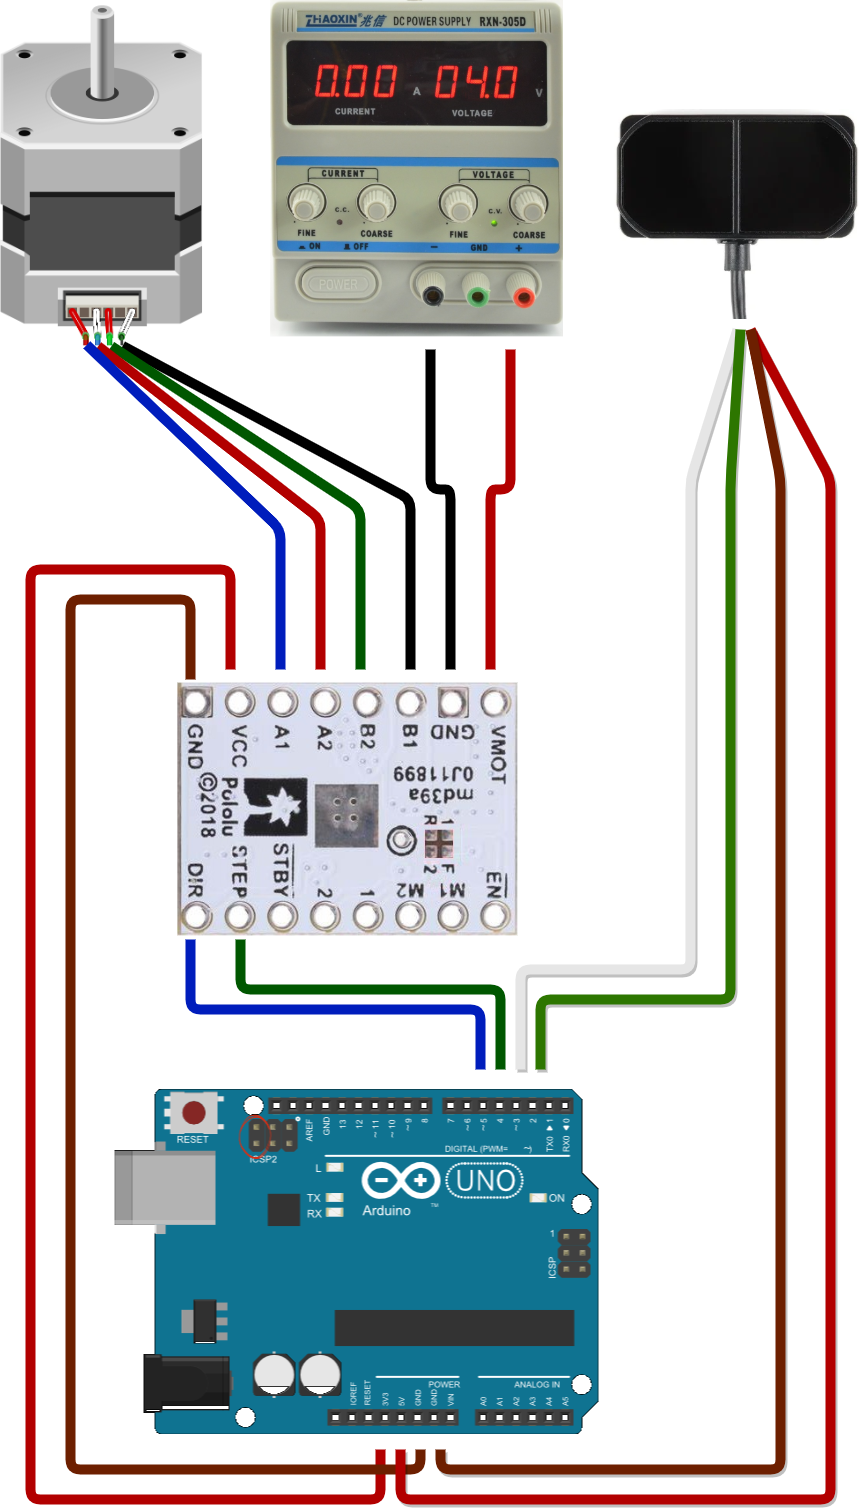
\includegraphics[scale=0.30]{lidar_2d_schemat}
    \caption{Schemat implementacji}
    \label{fig:lidar_2d_schemat}
\end{figure} 